\documentclass[a4paper]{article}
\usepackage[12pt]{extsizes} 
\usepackage[utf8]{inputenc}
\usepackage[english, russian]{babel}
\usepackage{setspace,amsmath}
\usepackage[left=20mm, top=15mm, right=15mm, bottom=15mm, nohead, footskip=10mm]{geometry} % настройки полей документа
\usepackage{multirow}
\usepackage{lipsum}
\usepackage{ amssymb }
\usepackage{amsmath, amstext}
\usepackage{siunitx}
\usepackage{subcaption}
\usepackage{wrapfig}
\usepackage{mathrsfs}	%символы
\usepackage{fancyhdr}   %колонтитулы
\usepackage{color, colortbl}	%цветные таблицы
\usepackage{adjustbox}
\usepackage{multirow}
\usepackage{enumerate, indentfirst, float}
\newcommand{\angstrom}{\textup{\AA}}


\newenvironment{bottompar}{\par\vspace*{\fill}}{\clearpage}



\begin{document} % начало документа

% НАЧАЛО ТИТУЛЬНОГО ЛИСТА
\begin{center}
\hfill \break
\Large{МИНИСТЕРСТВО ОБРАЗОВАНИЯ И НАУКИ РФ}\\
\vspace{0.6cm}
\large{ФЕДЕРАЛЬНОЕ ГОСУДАРСТВЕННОЕ АВТОНОМНОЕ \\ 
    ОБРАЗОВАТЕЛЬНОЕ УЧРЕЖДЕНИЕ ВЫСШЕГО\\
    ОБРАЗОВАНИЯ}\\
\vspace{0.9cm}
\centerline{\Large{\textbf{<<МОСКОВСКИЙ ФИЗИКО--ТЕХНИЧЕСКИЙ ИНСТИТУТ}}}

\Large{\textbf{(ГОСУДАРСТВЕННЫЙ УНИВЕРСИТЕТ)>>}}\\
\vspace{1.3cm}
\large{\textsf{Кафедра нанометрологии и наноматериалов}}\\
\vspace{1.2cm}
\Huge{\textbf{Рентгеновский дифрактометр}}\\
\vspace{0.5cm}
\large{Лабораторная работа по курсу:}\\
\bfseries \itshape \Large{<<Лабораторный практикум по нанодиагностике>>} \large
\end{center}

\vspace{2.5cm}
\null\hfill
\begin{minipage}{0.44\textwidth}
\large\textbf{Выполнили:}\\
Студенты 652-ой группы\\
\textsc{Марголин} Илья\\
\textsc{Нехаев} Александр\\
\textsc{Сёмкин} Валентин\\
\textsc{Серебренникова} Светлана\\
\textsc{Александров} Михаил\\
\textsc{Серягина} Екатерина\\
\textsc{Кружилин} Иван\\
\textsc{Еремеев} Даниил\\
\textsc{Тихонов} Сергей\\


\textbf{Дата выполнения работы:}\\
\textit{2019-ый год}\\
\end{minipage}\\
\vfill
\begin{center} \textsc{Долгопрудный 2019} \end{center}
\thispagestyle{empty} % выключаем отображение номера для этой страницы
% КОНЕЦ ТИТУЛЬНОГО ЛИСТА

\newpage
\tableofcontents
\newpage
\section{Задание}
\begin{enumerate}
    \item Построили спектр стандартного образца (корунд SRM1976a), идентифицировать отражения (по называнию найти его сертификат), выполнить профильный анализ (учесть при этом присутствие двух спектральных компонент Cu Kalpha меди). В данной работе у нас была трубка с медным анодом (длина волны около 0.154 нм). Указать неопределённости определения дифракционных максимумов.
    \item 	Сшить кривую рентгеновской рефлектометрии для заданной плёнки (сшивку начинать с области больших углов) оксида алюминия, обработать её в ПО Bede Refs, определить толщину плёнки, её плотность и шероховатости границ раздела. Плёнка $Al_2 O_3$ была выращена непосредственно на кремнии, поэтому модель простая-$Si/Al_2 O_3$. Плёнка оксида циркония была выращена на кремнии с естественным оксидом, затем отожжена, поэтому нужно задать модель вида $Si/SiO_2$ (около 2-8 нм) /$ZrO_2$. При моделировании учесть функцию прибора (угловую расходимость пучка можно определить по скану $\theta$. Образец 30 на 26 мм, радиус гониометра 26 см. Примерные параметры slits (щели на первичном пучке) можно взять из обработанной кривой (см. вложение)-их можно поварьировать.

    Для каждой подгруппы сравнить результат моделирования толщины плёнки $Al_2 O_3$ с приближением по периоду осцилляций (их много, можно учесть все)-при этом надо определить также экспериментальную ошибку.

\end{enumerate}


\newpage
\section{Практическая часть}
\subsection{Анализ дифракционного спектра образца корунда SRM1976a}
По полученным данным построим спектр стандартного образца (корунд SRM1976a) (рис. \ref{ris:ris1}). Проведем профильный анализ. Каждый из пиков спектра аппроксимируем распределением Войта: свёртка распределений Гаусса и Лоренца (см. Приложение рис. \ref{} - \ref{}). Пример анализа пика с наибольшей интенсивностью приведён на рис. \ref{ris:ris2}.

Проведем идентификацию отражения, сравнив результаты, полученные при обработке спектра, с опорными значениями из сертификата для SRM1976a. Результаты представлены в таблице \ref{tab1}.

\begin{figure}[h!]
		\begin{center}
			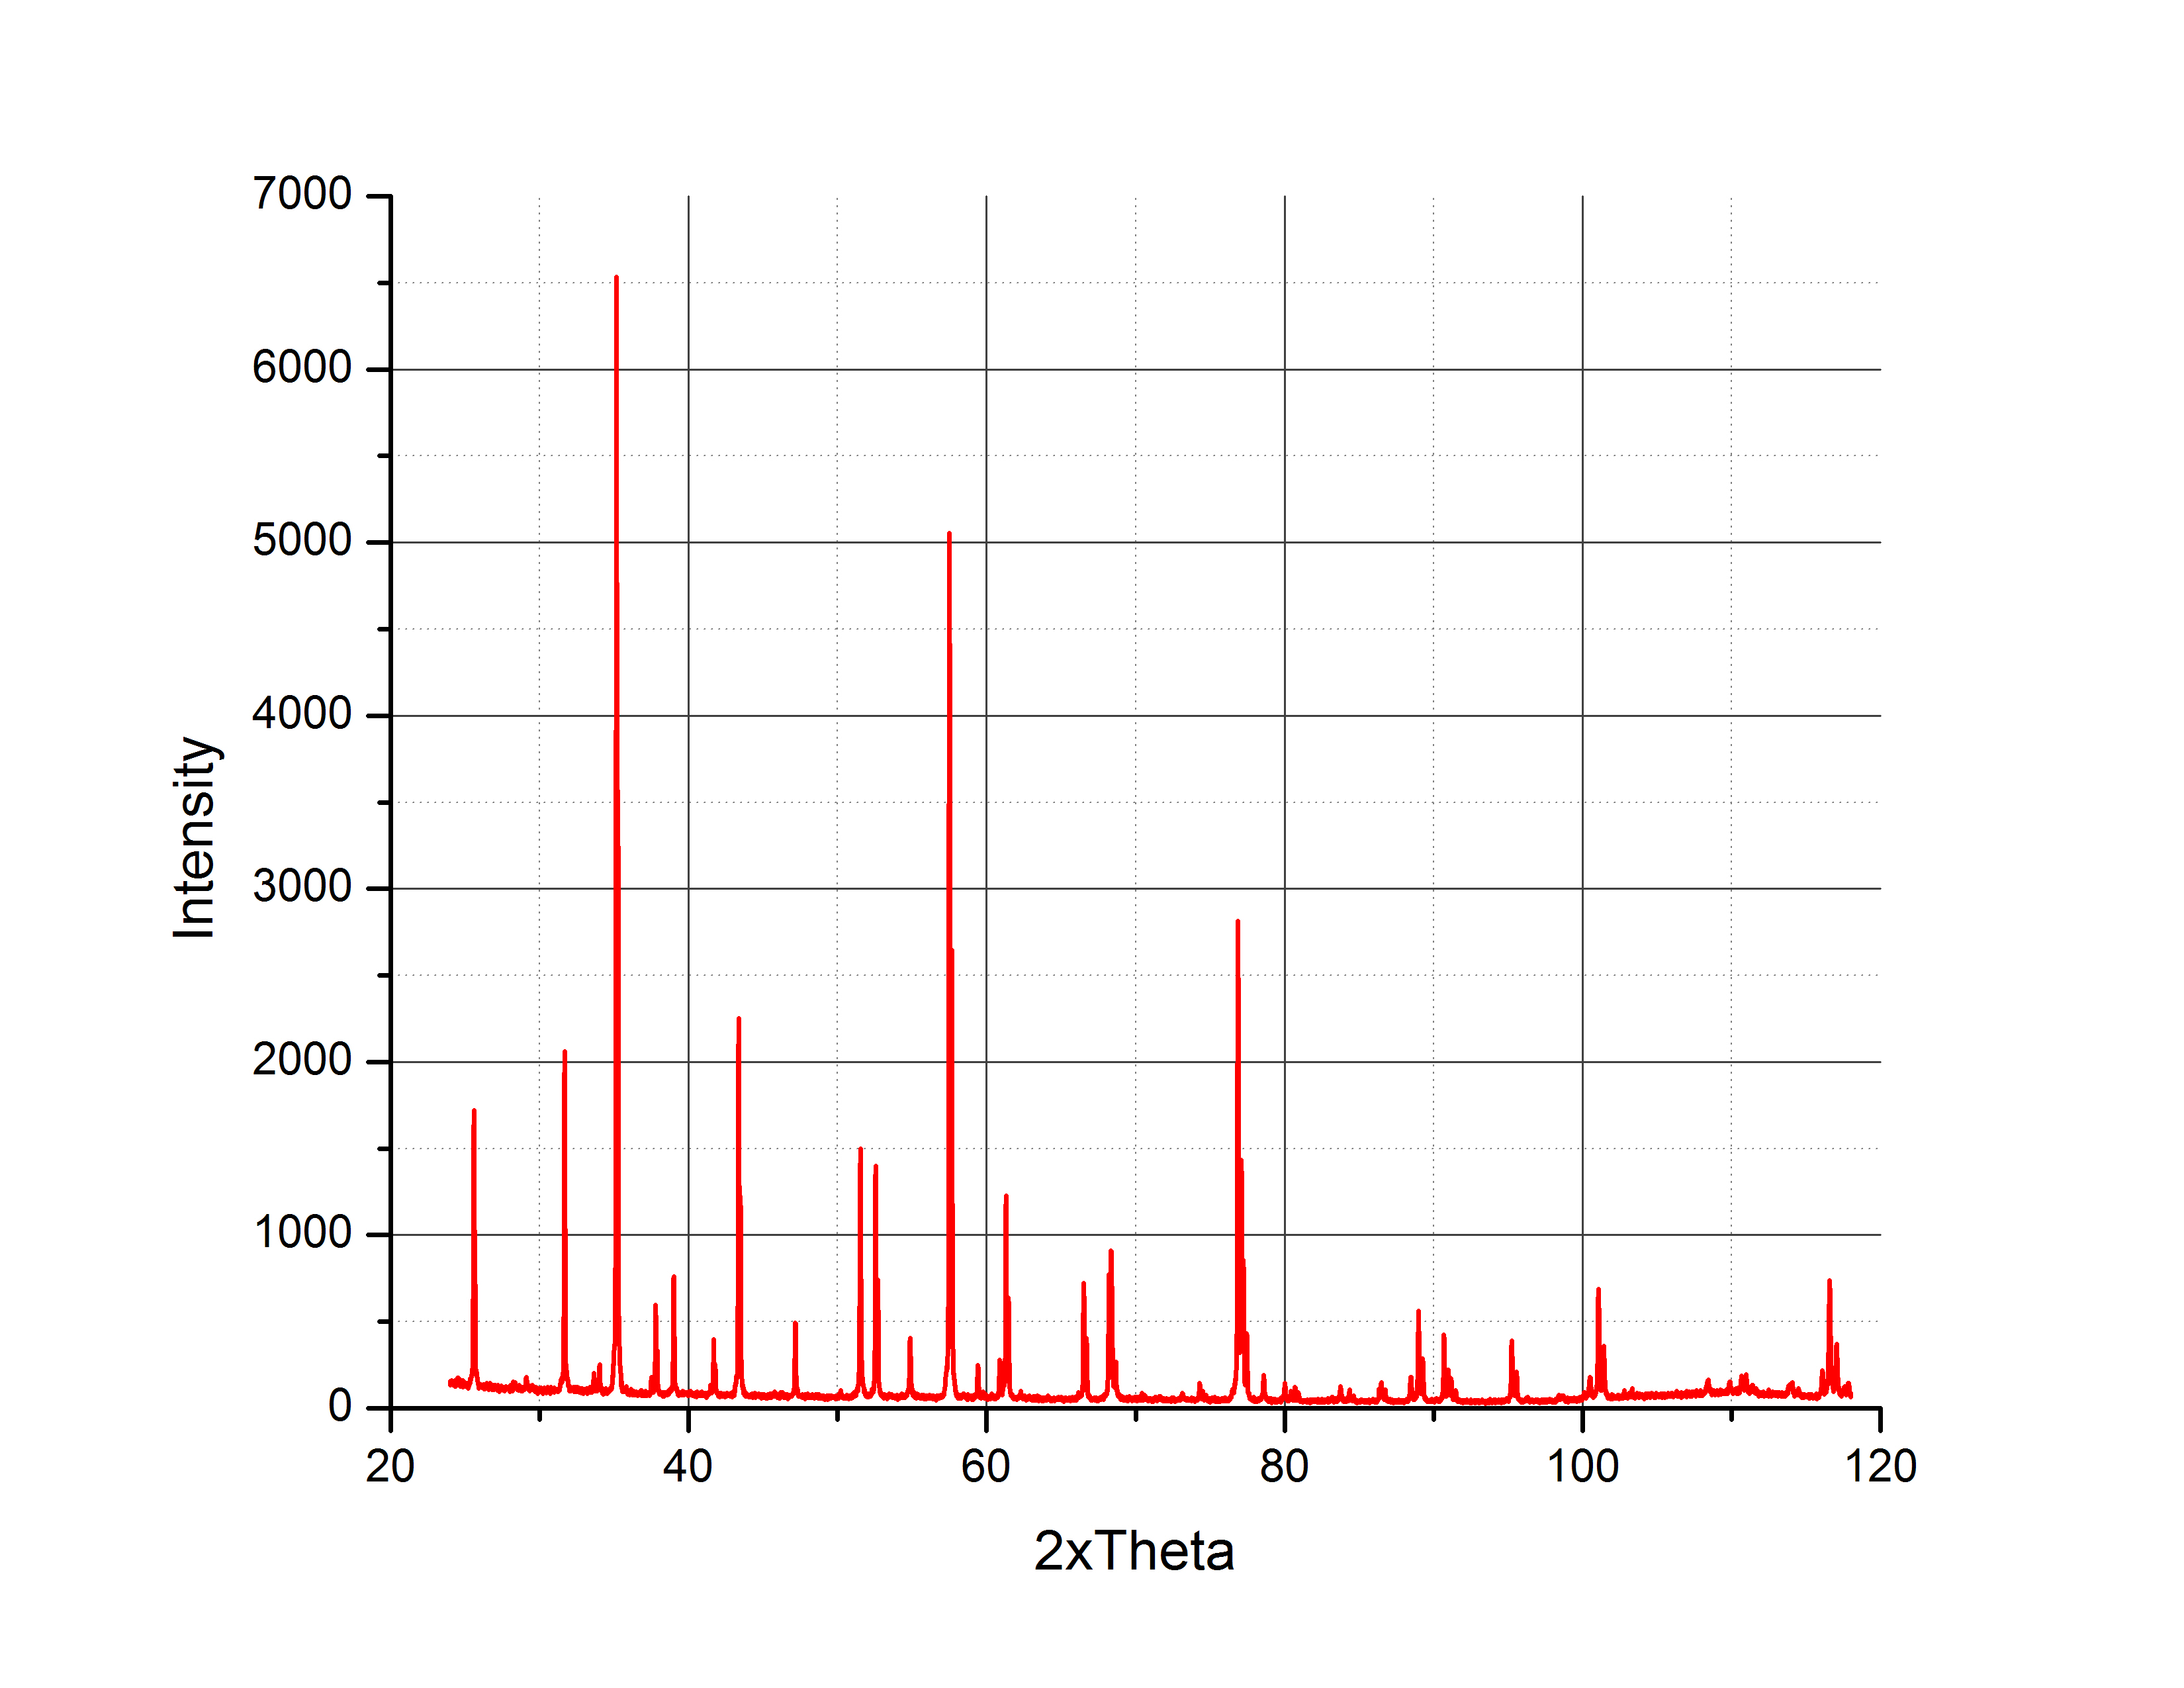
\includegraphics[scale = 0.65]{spec}
			\caption{Дифракционный спектр корунда}
			\label{ris:ris1}
		\end{center}	
	\end{figure}

	\begin{figure}[h!]
		\begin{center}
			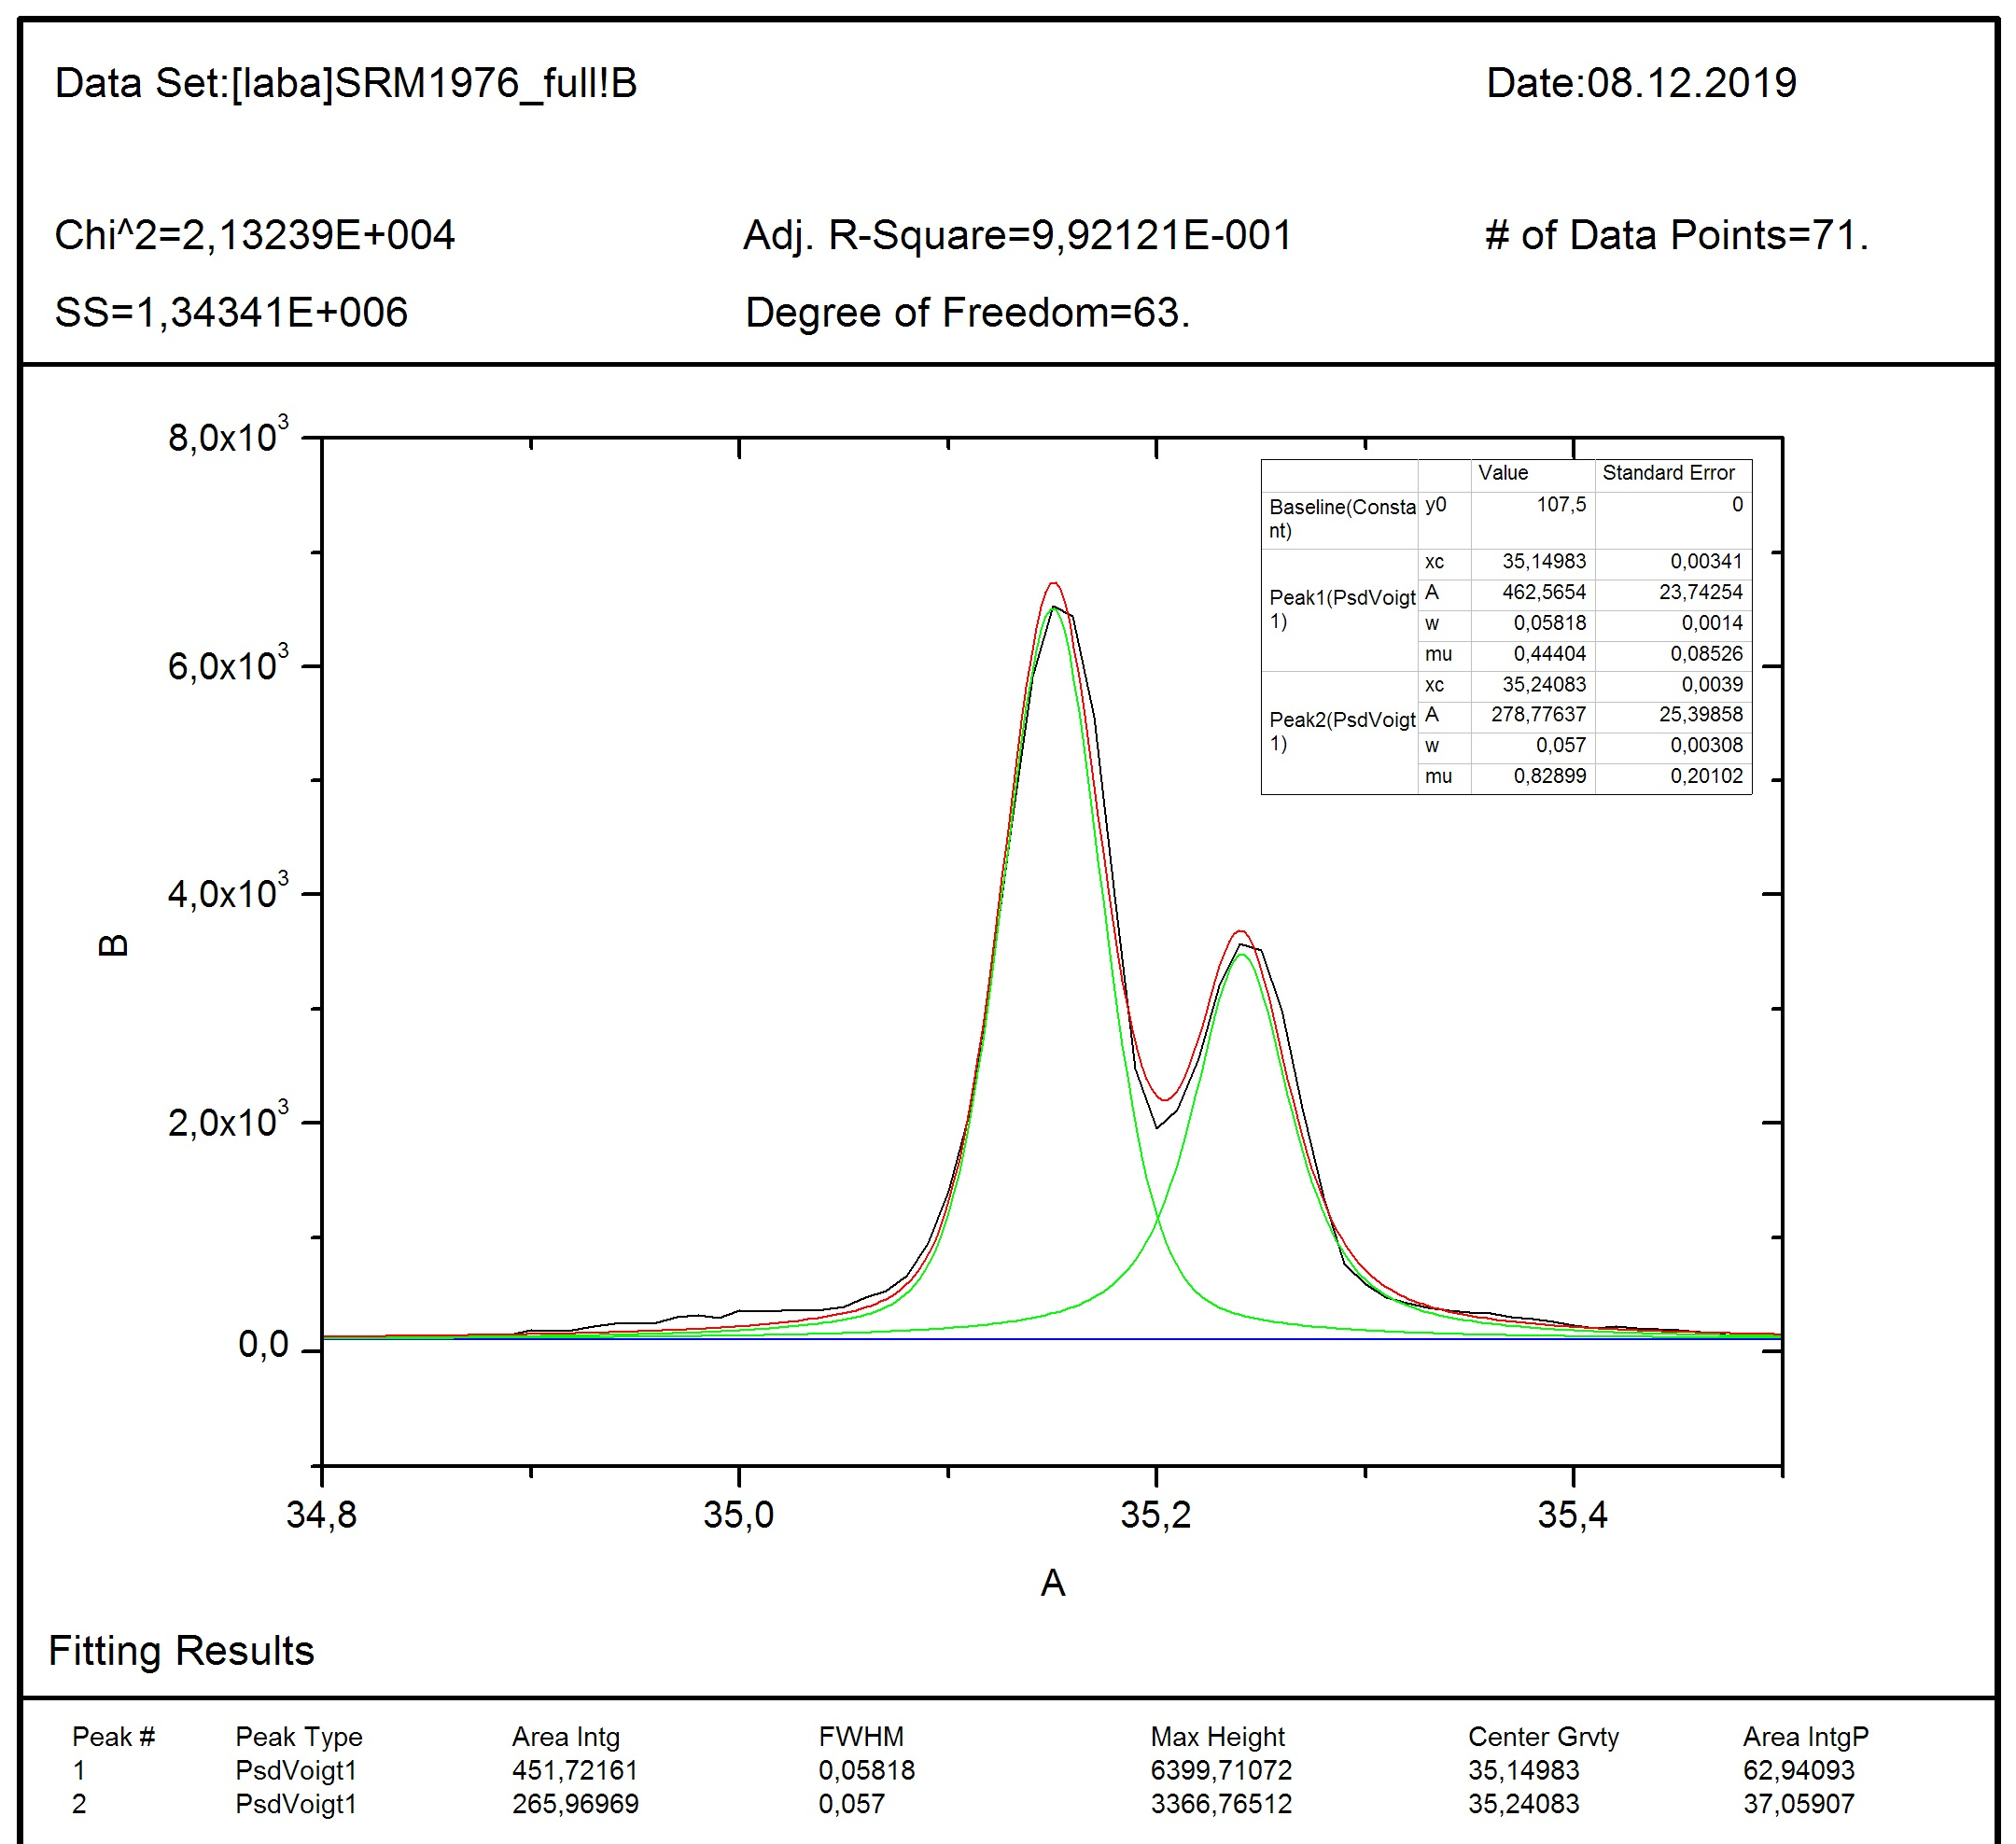
\includegraphics[scale = 0.8]{35deg_1}
			\caption{Theta = 35.150$^\circ$}
			\label{ris:ris2}
		\end{center}	
	\end{figure}

\begin{table}[h!]
		\centering
		\begin{tabular}{|c|c|c|}
			\hline
			\rowcolor[rgb]{0.86,1,1} $\Theta_{\text{experimental}}, ^\circ$& $\Theta_{\text{reference}}, ^\circ$ & $\text{Reflection}~(hkl)$\\
			\hline 
			 25.581 $\pm$ 0.009 & 25.575 & (012) \\
			 \hline 
			 35.150 $\pm$ 0.003& 35.147 & (104) \\ 
			 \hline 
			 37.782 $\pm$ 0.008& 37.775 & (110) \\ 
			 \hline 
			 41.681$\pm$ 0.015& 41.673 & (006) \\ 
			 \hline 
			 43.348$\pm$ 0.008& 43.351 & (113) \\ 
			 \hline 
			 52.550$\pm$ 0.010& 52.542 & (024) \\ 
			 \hline 
			 57.500$\pm$ 0.002& 57.495 & (116) \\ 
			 \hline 
			 61.300$\pm$ 0.013& 61.297 & (018) \\ 
			 \hline 
			 66.516$\pm$ 0.089& 66.515 & (214) \\ 
			 \hline 
			 68.202$\pm$ 0.027& 68.207 & (300) \\ 
			 \hline 
			 76.870$\pm$ 0.006& 76.866 & (1.0.10) \\ 
			 \hline 
			 77.230$\pm$ 0.012& 77.229 & (119) \\ 
			 \hline 
			 88.995$\pm$ 0.131& 88.989 & (0.2.10) \\ 
			 \hline 
			 90.704$\pm$ 0.106& 90.699 & (0.0.12) \\ 
			 \hline 
			 95.240$\pm$ 0.013& 95.242 & (2.2.6) \\ 
			 \hline 
			 101.060$\pm$ 0.984& 101.066 & (2.1.10) \\ 
			 \hline 
			 116.586$\pm$ 1.370& 116.091 & (324) \\ 
			 \hline 
			 116.093$\pm$ 2.851& 116.588 & (0.1.14) \\
			 \hline
		\end{tabular}
		\label{tab1}
	\end{table}
	\vspace{0.5pt}
	
\newpage

\subsection{Определение параметров элементарной ячейки} 

Положения пиков совпадают в пределах $0.4 \%$. По формуле Брегга-Вульфа:
$$2d\sin(\theta) = \lambda$$
Для погрешностей использовалась общая формула:

$$\Delta f = \dfrac{\partial f}{\partial x} \Delta x$$

\begin{itemize}
    
\item{Оксид рутения}
    
У оксида рутения тетрагональная решётка. Формулы для определения межплоскостного расстояния для тетрагональной решётки:
    
$$\dfrac{1}{d^2_{hkl}} = \dfrac{h^2}{a^2} + \dfrac{k^2}{b^2} + \dfrac{l^2}{c^2}$$
    
$$d_{110} = \dfrac{0.154 \text{ нм}}{2\sin(13.514)} = (3.295 \pm 0.013) \angstrom$$
    
$$d_{101} = \dfrac{0.154 \text{ нм}}{2\sin(17.635)} = (2.541 \pm 0.003) \angstrom$$
     
$$d_{210} = \dfrac{0.154 \text{ нм}}{2\sin(22.448)} = (2.017 \pm 0.005) \angstrom$$
      
Занесём рассчитанные параметры решётки в таблицу. В той же таблице укажем табличные значения:
      
\begin{table}[h!]
			\centering
			\begin{tabular}{|c|c|c|}
				\hline
				a & b & c\\
				\hline
				\multicolumn{3}{|c|}{Рассчитанные значения}\\
				\hline
				4.51 & 4.51 & 3.076\\
				\hline
				\multicolumn{3}{|c|}{Табличные значения}\\
				\hline
			\end{tabular}  
		\end{table}
    
    
    
    
    
    \item Рутений
\end{itemize}{}
\end{document}
